\documentclass[nofootinbib,twocolumn]{revtex4}
\pdfoutput=1
\usepackage{graphicx}
\usepackage{amsmath} 
\usepackage{amssymb}
\usepackage{bm}
\usepackage{hyperref}
\usepackage{todonotes}
\usepackage[normalem]{ulem}
\interfootnotelinepenalty=10000
\begin{document}

\begin{titlepage}
   \begin{center}
       \vspace*{1cm}

       \LARGE\textbf{Scalar Radiation from Symmetron Field Oscillations}

       \vspace{0.5cm}
        \normalsize PIC1 Scientific Project
            
       \vspace{1.5cm}

       \large \textbf{Sebastião Fonseca}

       \vfill
            
       \normalsize Under the supervision of Javier Rubio
            
       \vspace{10cm}
     
       
\includegraphics[width=0.4\textwidth]{Images/ist.png}
       
       %\vspace{1.5cm}
            
       Department of Physics\\
       Instituto Superior Técnico\\
       Portugal\\
       25/06/2022
       
       \vspace{5cm}
       

   \end{center}
\end{titlepage}

\title{\large \bf  Scalar radiation from symmetron field oscillations}
%\date{\today}
\author{Sebastião Fonseca}
\affiliation{{Departamento de Física, Instituto Superior Técnico - IST,
Universidade de Lisboa - UL,
Av. Rovisco Pais 1, 1049-001 Lisboa, Portugal}}

\begin{abstract}
\vspace{0.5cm}
In recent years, modified theories of gravity have emerged as a possible explanation for the accelerating rate of expansion of the Universe. These theories rely on screening mechanisms is order to hide from local gravity tests, which naturally makes them harder to detect.
In this paper we study the behaviour of the symmetron field around massive objects. After obtaining the time independent static solution, small time dependent perturbations are introduced in the form of radial oscillations. These oscillations result in the object emitting scalar radiation into the surrounding space which could be an avenue through which we could test the existence of the symmetron. Finally, the relative power radiated by a compact object similar to the sun was calculated to be $\frac{1}{E}\frac{dE}{dt}\approx O(10^{-19})s^{-1}$.
\vspace{0.5cm}
\end{abstract}

\maketitle

%%%%%%%%%%%%%%%%%%%%%%%%%%%%%%%%%%%%%%%
\section{Introduction}
%%%%%%%%%%%%%%%%%%%%%%%%%%%%%%%%%%%%%%%

It is a well established fact that the Universe is expanding at an accelerating rate \cite{SupernovaSearchTeam:1998fmf}.
In the standard model of cosmology, the $\Lambda$CDM (Lambda Cold dark matter) model, this acceleration is explained by a cosmological constant $\Lambda$ in the Einstein equations \cite{Carroll:2000fy}. However, in recent years, there has been interest in studying alternative explanations for this expansion \cite{Armendariz-Picon:2000nqq,Carroll:2003wy}, such as previously undetected scalar fields \cite{Joyce:2014kja,Silvestri:2009hh} in modified theories of gravity. 

One would expect that a new scalar degree of freedom would introduce a new, fifth force which would alter the strength of gravity. However, many high precision tests of General Relativity \cite{Will:2014kxa} have been conducted and no evidence of such a fifth force has been found. In fact, if such a fifth force exists, it must be either short ranged, as the inverse square law has been proven to hold even for distances at millimeter scales \cite{Will:2014kxa,Westphal:2020okx}; or it must be much weaker than gravity. All these experiments are, however, conducted near our solar system. It has been realised that these tests do not rule out the possibility of a long range fifth force that could be suppressed in smaller scales so that local gravity tests hold true. This suppressing effect has been referred to as a screening mechanism, and regions where this effect is active are said to be screened. Therefore, if these scalar fields were to exist, then they would have to be hidden through a screening mechanism \cite{Brax:2012gr,Burrage:2017qrf} in order to satisfy local fifth force constraints. This mechanism would have to decouple the fields from matter, making them undetectable near high density environments. However, in low density environments, the screening effect would be deactivated and the fields would couple to matter with gravitational strength.

Naturally, then, the question arises on how we could go about detecting these fields. In General Relativity, it is well known that radial oscillations of compact objects do not cause the emission of gravitational waves \cite{Barausse:2021pwx}. However, it has been proposed that, in modified theories of gravity, due to the coupling of these fields to mass, radially pulsating objects could carry perturbations into their surrounding space \cite{Sotani:2014tua}. This means that pulsating sources could emit (scalar) gravitational waves, and events such as stellar collapse could be sources for these waves \cite{Bezares:2021yek}. In addition, systems such as binary star systems or binary pulsars, whose tidal forces can cause radial perturbations, would be sources for the emission of these scalar gravitational waves, which would cause deviations from General Relativity which could potentially be tested by gravitational wave detectors \cite{Barausse:2021pwx}.

In this paper, we will study this possibility for simple compact objects in a non-relativistic approximation. Similar work has been done with other screening mechanisms, such as the so-called chameleon screening \cite{Khoury:2004,Silvestri:2011ch}, however, we will focus solely on the symmetron mechanism, proposed in Ref.~\cite{Hinterbichler:2010es}. 

The symmetron screening mechanism works by combining a symmetry breaking potential with a coupling to the local mass density. In regions of low density, the broken symmetry of the potential results in the scalar field obtaining a non-zero vacuum expectation value (vev) which mediates a fifth force with comparable strength to gravity. However, in regions of high mass density, the symmetry of the effective potential is restored due to the coupling of the field to matter, the vev goes to zero, and the screening effect is activated. In the next section we shall go over its behaviour in more detail.

This paper is organized as follows. In Section \ref{sec2}, we will do a brief introduction to the symmetron mechanism, its governing equations and  behaviour, as well as the configuration of the system we will be working with. In Section \ref{sec3} we obtain a static profile to be used as a background for our work in Section \ref{sec4}, where we introduce perturbations into the system and obtain the time dependent perturbation profile. Next, in Section \ref{sec5}, having obtained the ripples in the symmetron field, we are able to calculate the relative power emitted by the object as scalar radiation. Finally, in Section \ref{sec6} we discuss the results obtained and the future outlook of this work.

%In this paper we have used metric signature $(-,+,+,+)$ and used natural units, where $c = \hbar = 1$

%%%%%%%%%%%%%%%%%%%%%%%%%%%%%%%%%%%%%%%
\section{The Model}\label{sec2}
%%%%%%%%%%%%%%%%%%%%%%%%%%%%%%%%%%%%%%%

For the symmetron screening mechanism to work, the vev must be low in regions of high mass density, but become large in regions of high mass density.
This is achieved by the combination of a symmetry breaking potential \cite{Hinterbichler:2011ca}

\begin{equation}
    V(\phi) = -\frac{1}{2}\mu^2\phi^2+\frac{1}{4}\lambda\phi^4,
\end{equation}
with square mass $\mu^2>0$ and self-interaction $\lambda>0$ and a universal coupling to the trace of the matter stress-energy tensor, such that the local matter density contributes to the effective mass of the field.
The associated action is given by \cite{Hinterbichler:2010es} 
\begin{multline}
        S = \int d^4x \sqrt{-g}\left[\frac{M_{Pl}^2}{2}R - \frac{1}{2}(\partial\phi)^2-V(\phi) \right] \\
   + \int d^4x \mathcal{L}_m[\Tilde{g}],
   \label{Action}
\end{multline}
with $M_{Pl} = \sqrt{8\pi G}^{-1}$ being the Planck mass, $R$ the curvature scalar and $\sqrt{-g}$ the square root of the determinant of the metric tensor, using signature $(-,+,+,+)$.
Here, $\mathcal{L}_m$ is the Lagrangian of the matter fields, coupled to the Jordan frame metric
\begin{equation}
    \Tilde{g}_{\mu\nu} \equiv A^2(\phi)g_{\mu\nu}\,,
\end{equation}
with $g_{\mu\nu}$ the Einstein metric.
The equation of motion for the field then becomes
\begin{equation}
    \Box\phi = \partial_{\phi} V - A^3(\phi)(\partial_{\phi} A)\Tilde{T},
    \label{EOM1}
\end{equation}
%\todo[inline]{What is $\Box$?}
where $\Tilde{T} = \Tilde{T}_{\mu\nu}\Tilde{g}^{\mu\nu}$ is the trace of the matter stress-energy tensor  and $\Box$ is the d'Alembert operator. For non-relativistic matter, $\Tilde{T} \approx -\Tilde{\rho}$, $\rho$ being the mass-energy density.
Rewriting Eq.~\eqref{EOM1} in terms of $\rho \equiv A^3(\phi)\Tilde{\rho}$, we attain the equation of motion for the field
\begin{equation}
    \Box\phi = \partial_{\phi} V + (\partial_{\phi} A)\rho.
    \label{FullEOM}
\end{equation}
~~For the simplest symmetron theories, $A(\phi)$ takes the form of a quadratic coupling \cite{Hinterbichler:2011ca}
\begin{equation}
    A(\phi) = 1+\frac{\phi^2}{2M_s^2}+\mathcal{O}\left(\frac{\phi^4}{M_s^4}\right),
\end{equation}
where $M_s$ is a mass term which controls the strength of the screening effect, the higher its value, the higher the local density needs to be in order to trigger the screening mechanism. We will also soon see that we can safely ignore higher order terms of $\left(\phi^2 / M_s^2\right)$.

Therefore, for an environment with roughly homogeneous density $\rho$, the field is governed by the effective potential
\begin{equation}\label{Veff}
    V_{\rm eff}(\phi) = \frac{1}{2}\left(\frac{\rho}{M_s^2}-\mu^2 \right)\phi^2 +\frac{1}{4}\lambda\phi^4.
\end{equation}
~~Inside massive objects, such that $\rho \gg \mu^2M_s^2$, the field obtains a vev equal to 0, and the field is suppressed by the presence of a massive object. However, far away from these objects, where $\rho \ll \mu^2M_s^2$, the $\mathbb{Z}_2$ symmetry $\phi \to -\phi$ is spontaneously broken, the vev now goes to $\phi_{\infty} \equiv \frac{\mu}{\sqrt{\lambda}}$ and the field is no longer suppressed by the massive object.

The effective potential \eqref{Veff} involves two mass terms, $\mu$ and $M_s$, and one dimensionless coupling term $\lambda$.
In order to find numerical values for these terms, we will introduce some constraints. Firstly, in order to induce the symmetry breaking, we need the field to have negative mass around the current cosmic density, which happens at a critical value $\rho = \mu^2M_s^2$. From the Friedmann equation, we have 
\begin{equation}
    H_0^2 \sim \frac{\rho}{M_{Pl}^2},
    \label{Friedmann}
\end{equation}
where $H_0$ is the Hubble constant and we have omitted a factor of $1/3$ as we are only interested in orders of magnitude. This then gives us the condition $H_0^2 M_{Pl}^2 \sim \mu^2 M_s^2$, or, equivalently
\begin{equation}
    \mu \sim \frac{M_{Pl}}{M_s}H_0.
    \label{constaint 1}
\end{equation}
~~Since small fluctuations $\delta\phi$ around $\phi_{\infty}$ couple as \cite{Hinterbichler:2010es}
\begin{equation}
    \sim \frac{\phi_{\infty}}{M_s^2}\delta\phi\rho,
\end{equation}
and we want this new force to be comparable to gravity, this means $\frac{\phi_{\infty}}{M_s^2} \sim \frac{1}{M_{Pl}}$, therefore
\begin{equation}
    \phi_{\infty} \equiv \frac{\mu}{\sqrt{\lambda}} \sim \frac{M_s^2}{M_{Pl}}.
    \label{midconstraint}
\end{equation}
~~Combining Eq.~\eqref{midconstraint} with Eq.~\eqref{constaint 1}, we get a constraint for the value of $\lambda$
\begin{equation}
    \lambda \sim \frac{M_{Pl}^4H_0^2}{M_s^6}.
    \label{constraint 2}
\end{equation}
~~And lastly, in order so satisfy the constraints imposed by local gravity tests, we also require that $M_s < 10^{-4}M_{Pl}$, as shown in Ref.~\cite{Hinterbichler:2011ca}. Therefore, from Eq.~\eqref{midconstraint}, we find that $\phi_{\infty} \lesssim 10^{-4}M_s$, hence we can safely ignore higher order terms of $\left(\phi^2 / M_s^2\right)$ as previously stated.

%%%%%%%%%%%%%%%%%%%%%%%%%%%%%%%%%%%%%%%
\subsection{The configuration}
%%%%%%%%%%%%%%%%%%%%%%%%%%%%%%%%%%%%%%%

We want to study the behaviour of the symmetron near a radially pulsating compact object, whose pulsations can be caused, for example, by the tidal forces exerted on it by its pair in a binary system or by the object crossing the galactic halo. Naturally, these systems are very complex, so, in order to simplify our problem, we will be making a few approximations: 

\begin{enumerate}
\item We will be working in the Newtonian limit, where the metric can be well approximated by the flat Minkowski metric, $\eta_{\mu\nu}$, and the curvature scalar $R$ is null. Additionally, we will be ignoring relativistic effects.
\item The object we are modeling is a perfectly spherical compact object with similar dimensions as an average star. This object has constant density $\rho_c$ and radius $R_c$ (when unperturbed).
\item We will approximate the deformations caused by tidal forces as radial pulsations with amplitude $\Delta R$ and constant frequency $\omega $ such that 
\begin{equation}
R(t) = R_c + \Delta R \sin(\omega t)\,.    
\end{equation}
\item The region surrounding the object is a perfect vacuum where the density $\rho = 0$, such that
\begin{equation}
\rho_0(r) = \rho_c\, \Theta\left(1-\frac{r}{R_c}\right),    
\end{equation}  
where $\Theta(x)$ is the Heaviside step function.
\end{enumerate}

With these assumptions, we can now start solving the equations of motion of the system. First we will solve the time-independent case in order to compute the static profile for the symmetron field. Next, we will introduce the radial pulsations and study the resulting time dependent oscillations of the field. Finally, from these oscillations, we will obtain the energy loss rate due to symmetron field oscillations. For the sake of concreteness, we will consider a compact object with similar compactness to the Sun,
$\rho_c \sim 10^{-18}$ GeV$^4$ and $R_c  \sim 10^{24}$ GeV. For the oscillation parameters, we will be using $\omega ={R^{-1}_c}$ and choosing $\Delta R_c = 0.01R_c$, as tidal deformations in binary systems can cause radial discrepancies of up to 1$\%$ \cite{Fabry_2022}. As for the symmetron's coefficients, from Eq.~\eqref{constaint 1} and Eq.~\eqref{constraint 2}, and setting $M_s \sim 10^{14}$ GeV, we obtain $\mu \sim 10^{-38}$ GeV and $\lambda \sim 10^{-92}$.

%%%%%%%%%%%%%%%%%%%%%%%%%%%%%%%%%%%%%%%
\section{\label{sec3}The Static Profile} 
%%%%%%%%%%%%%%%%%%%%%%%%%%%%%%%%%%%%%%%

We first begin by obtaining the field profile for a time independent static solution  $\phi_0$. Working in spherical coordinates, the equation of motion in this case becomes
\begin{equation}
    \frac{d^2\phi_0}{dr^2} + \frac{2}{r}\frac{d\phi_0}{dr} = \left(\frac{\rho_0}{M_s^2}-\mu^2 \right)\phi_0 +\lambda\phi_0^3.
    \label{EOMStatic}
\end{equation}
~~This equation cannot be solved analytically. However, we can simplify it by approximating the potential as quadratic around each minima of the potential as such
\begin{equation}
    V(\phi) = \left\{
\begin{array}{ll}
      \frac{1}{2}m_c^2\phi^2, & \hspace{5mm} r<R_c\,,\\
      \frac{1}{2}m_0^2(\phi-\phi_{\infty})^2, & \hspace{5mm} r>R_c \,, \\
\end{array} 
\right. 
\end{equation}
where 
\begin{equation}
m_c = \sqrt{\frac{\rho_c}{M_2^2}-\mu^2}   \hspace{5mm}  \textrm{and}   \hspace{5mm}  m_0 = \sqrt{2}\mu,
\end{equation} 
are respectively the mass of the field inside and outside the object. In this approximation, the equation of motion becomes 
\begin{equation}\label{eqBackground}
\frac{d^2\phi_0}{dr^2} + \frac{2}{r}\frac{d\phi_0}{dr} = \left\{
\begin{array}{ll}
      m_c^2\phi, & \hspace{5mm} r<R_c\\
      m_0^2(\phi-\phi_{\infty}), & \hspace{5mm} r>R_c \,. \\
\end{array} 
\right. 
\end{equation}
%which is much simpler to solve.
In order to avoid singularities at $r=0$, our first boundary condition will be $\frac{d}{dr}\phi_0(0) = 0$, and, since we want the field to converge to $\phi_{\infty}$ far away from the object, our second boundary condition becomes $\lim_{r\rightarrow\infty}\phi_0(r) = \phi_{\infty}$.
Solving Eq.~\eqref{eqBackground} with these conditions gives us
\begin{equation}\label{eqphir}
\phi_0(r) = \left\{
\begin{array}{ll}
      \frac{A}{r}\sinh\left(m_cr\right), & \hspace{5mm}r<R_c\\
     \frac{B}{r}e^{-m_0 r}+\phi_{\infty}, & \hspace{5mm}r>R_c \, . \\
\end{array} 
\right. 
\end{equation}
\begin{figure}[t]
    \centering
    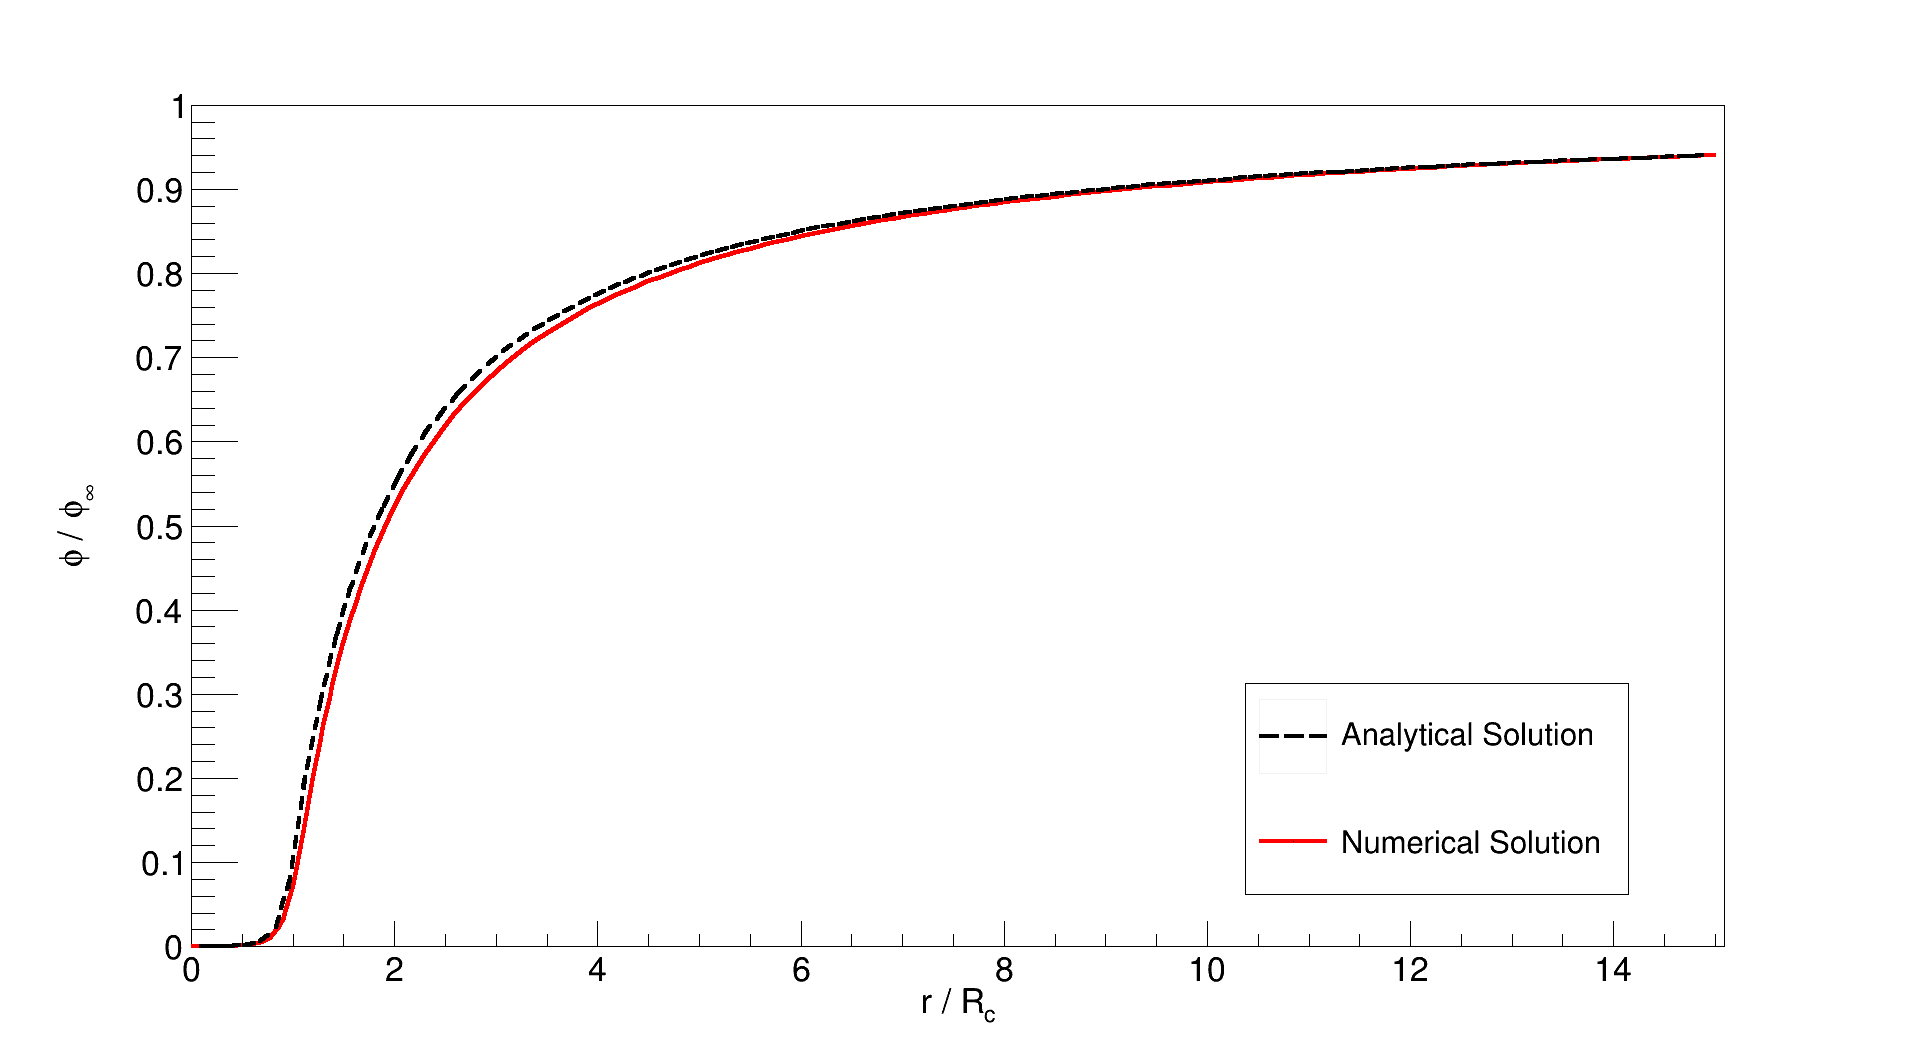
\includegraphics[width=1\columnwidth]{Images/Static.png}
    \caption{The symmetron field profile ($\varphi$) for a static object as a function of $x=\frac{r}{R_c}$. We can see that the approximate analytical solution (black) is very similar to the numerical solution (red). We can clearly see the screening mechanism at work, as the field is suppressed in the high density environment, when $x<1$. }
    \label{Static}
\end{figure}
with $A$ and $B$ two integration constants which can be obtained by matching the field and its first derivative at $r=R_c$. For a large object, they take the form \cite{Hinterbichler:2010es}
\begin{equation}
    A = \phi_{\infty}\frac{2R_c}{\sqrt{\alpha}}e^{-\sqrt{\alpha}}
    \quad\mathrm{;}\quad 
    B = \phi_{\infty}R_c\left(\frac{1}{\sqrt{\alpha}}-1\right),
\end{equation}
where 
\begin{equation}
\alpha \equiv \frac{\rho_c R_c^2}{M_s^2} = 6\frac{M_{Pl}^2}{M_s^2}\Phi    
\end{equation} 
is a constant which measures the strength of the Newtonian potential at the surface of an object.

We can now verify the validity of this approximation by solving the equation numerically.
To this end, it is convenient to use dimensionless units
\begin{equation}
 x \equiv \frac{r}{R_c}\,, \hspace{10mm}    \varphi \equiv \frac{\phi}{\phi_{\infty}}\,.
\end{equation}
~~Plugging these into Eq.~\eqref{EOMStatic} and simplifying we get 
\begin{equation}
    \frac{d^2\varphi_0}{dx^2} + \frac{2}{x}\frac{d\varphi_0}{dx} = R_c^2\left[\left(\frac{\rho_0}{M_s^2}-\mu^2 \right)\varphi_0 +\mu^2\varphi_0^3\right],
\end{equation}
which we solve with the same boundary conditions as before. The result is displayed in Figure \ref{Static}, showing an excellent agreement with the analytical approximation \eqref{eqphir} and clearly illustrating the screening mechanism. 
Inside the object, for $x<1$, the symmetron is screened and is undetectable. However, outside the object, the coupling is turned back on and the field very quickly approaches $\phi_{\infty}$. 

%%%%%%%%%%%%%%%%%%%%%%%%%%%%%%%%%%%%%%%
\section{\label{sec4}Time-dependent Profile}
%%%%%%%%%%%%%%%%%%%%%%%%%%%%%%%%%%%%%%%

Having obtained the background solution $\phi_0$, we can now introduce the perturbations into the system
\begin{equation}
    \phi(r,t) = \phi_0(r) + \delta\phi(r,t)
    \quad\mathrm{;}\quad 
     R(t) = R_c + \delta R(t).
\end{equation}
%\todo[inline]{ Also what follows till the end of the column is too telegraphic...This is the most important part of the paper!!!}
Density, in our approximation that the object is perfectly spherical, is given by
\begin{equation}
\rho = \frac{M}{\frac{4}{3}\pi R^3}   \,, 
\end{equation}
plugging in $R(t)$, assuming $\delta R \ll R $ and linearizing we get
\begin{equation}
    \rho(r,t) =\rho_0\left[1-3\frac{\delta R}{R_c}\right] = \rho_0(r)+\delta\rho(r,t),
\end{equation}
where 
\begin{equation}
\delta\rho(r,t) = -3\rho_c\frac{\Delta R}{R_c} \sin(\omega t)\Theta(1-\frac{r}{R_c})\,.
\end{equation}
~~Since $\sin(\omega t)$ is periodic, we can ignore the negative sign.

Plugging the perturbations into Eq.~\eqref{FullEOM} we obtain
\begin{equation}
    \Box\phi_0 + \Box\delta\phi = \left( \frac{\rho_0+\delta\rho}{M_{s}^2}-\mu^2\right)(\phi_0 + \delta\phi)+\lambda(\phi_0 + \delta\phi)^3.
\end{equation}
~~Once again we use the same dimensionless units when solving this equation, $x$ and $\varphi$, as well as rescaled time variable $\tau \equiv t/R_c$. 
Finally, after simplifying and linearizing the equation, we get 
\begin{equation}
    \Tilde{\Box}\delta\varphi = R_c^2\left[\frac{\delta\rho}{M_{s}^2}\varphi_0+\left(\frac{\rho_0}{M_{s}^2}-\mu^2 \right)\delta\varphi+3\mu^2\varphi_0^2\delta\varphi\right],
    \label{FinalEOM}
\end{equation}
where $\Tilde{\Box}$ is the d'Alembert operator rewritten in normalized units.

We are assuming the field is completely unperturbed at $\tau=0$, therefore we will use initial conditions $\delta \varphi (x,0) = \partial_{\tau}\delta \varphi (x,0) = 0$. As for boundary conditions, there should be no oscillations at $r=0$, nor do we expect these perturbations to propagate to infinity, so we choose the conditions $\lim_{x \to (0 , \infty)} \delta \varphi(x,\tau) = 0$.

%%%%%%%%%%%%%%%%%%%%%%%%%%
\begin{figure}[ht]
    \centering
    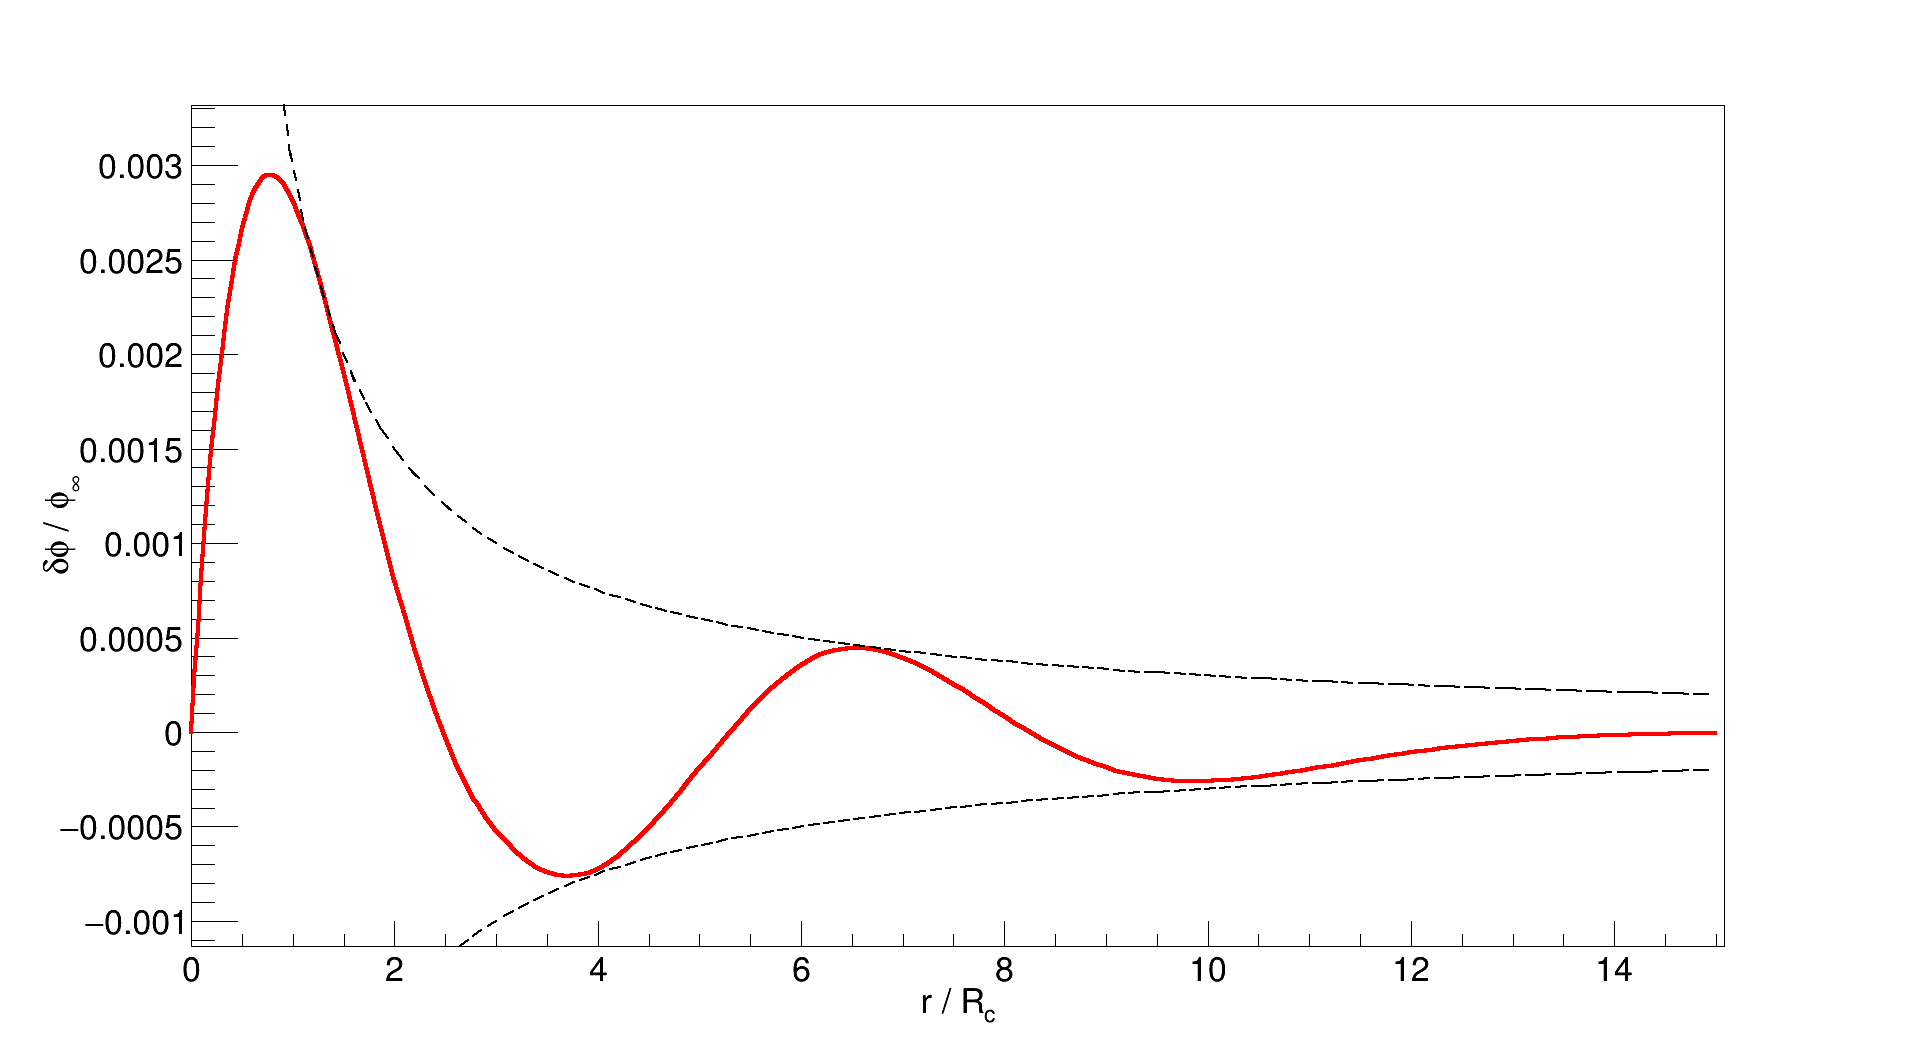
\includegraphics[width=1\columnwidth]{Images/P_t11.png}
    \caption{The symmetron perturbation field profile $\delta\varphi$ near a pulsating object as a function of $x = \frac{r}{R_c}$ at $t = 11R_c$ (red) and the functions $\pm \delta\varphi(1)/x$ (black). We can see that the the waves emitted by the object decay with $\frac{1}{x}$, as expected for a spherical source.   }
    \label{ProfileT6}
\end{figure}
%%%%%%%%%%%%%%%%%%%%%%%%%%
\begin{figure}[ht]
    \centering
    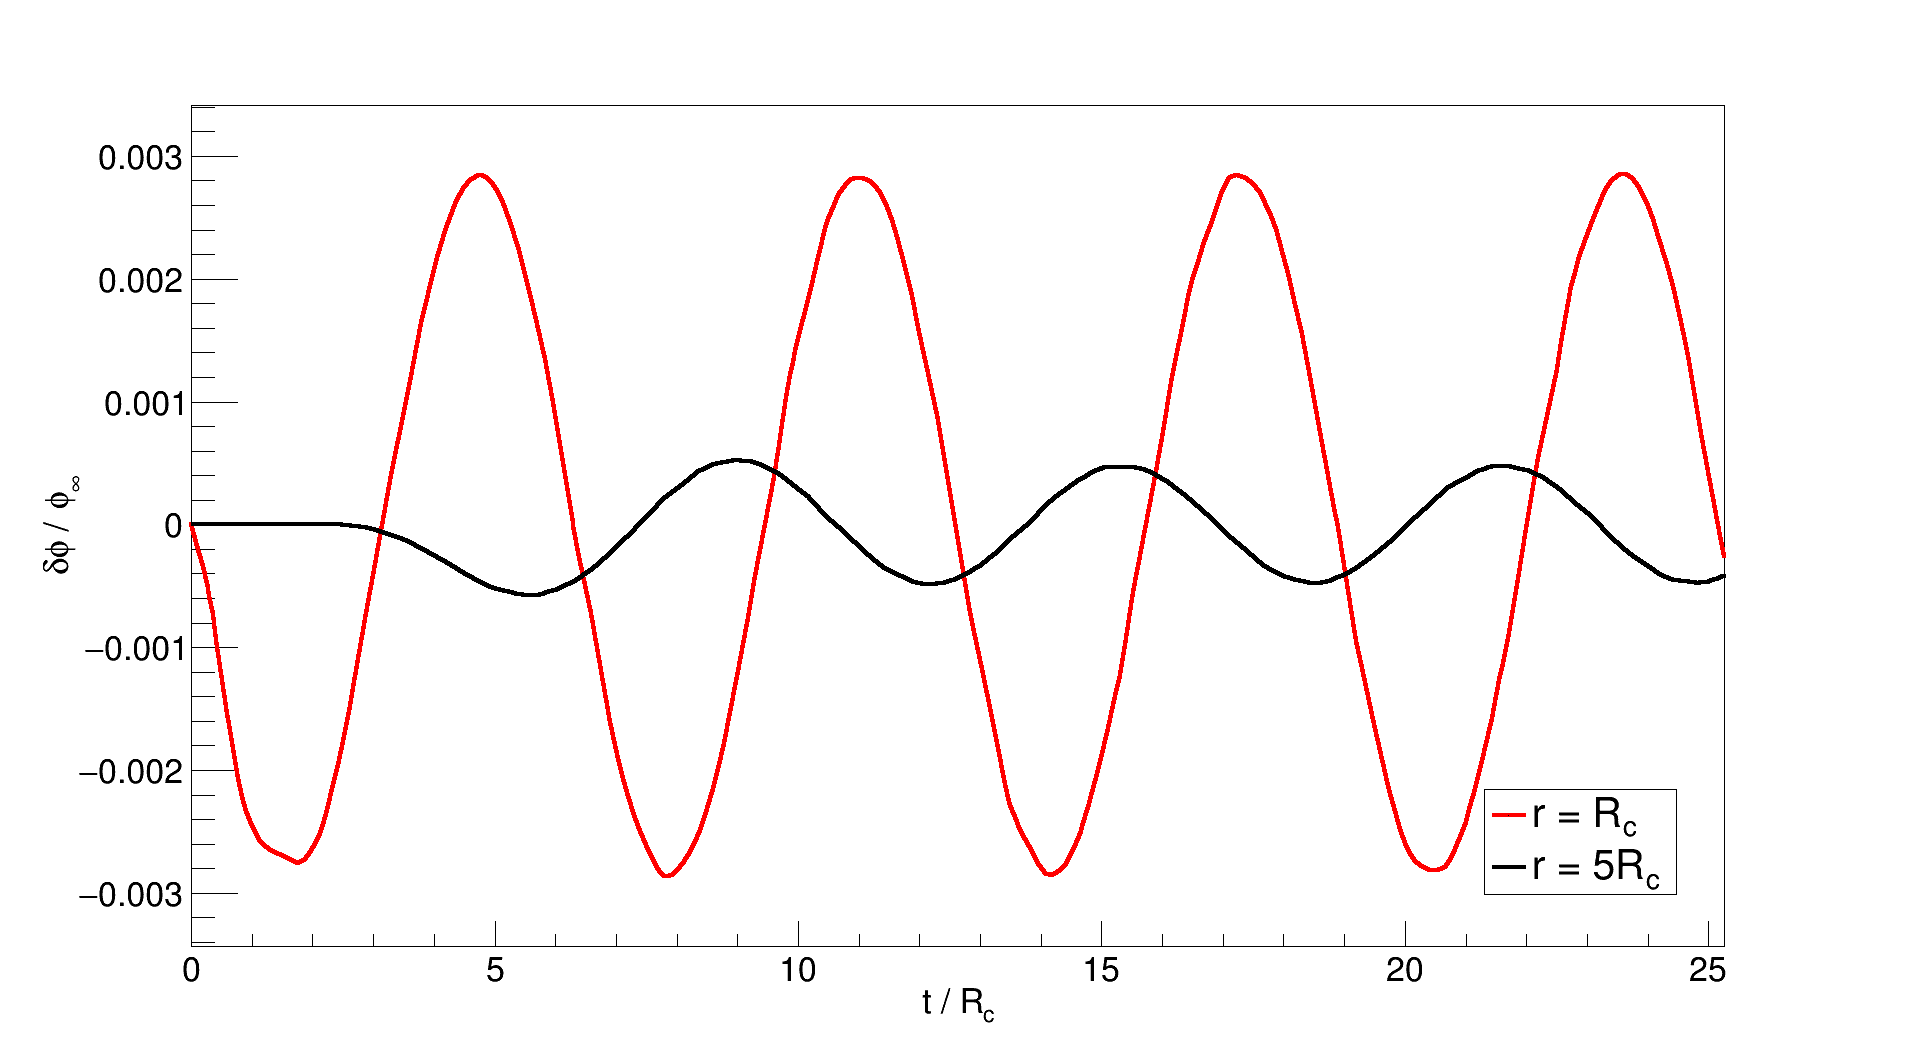
\includegraphics[width=1\columnwidth]{Images/P_r.png}
    \caption{The symmetron perturbation field profile $\delta\varphi$ near a pulsating object at as function of $\tau = \frac{t}{R_c}$ at radius $R_c$ (red) and $5R_c$ (black). It is also worth noting that these waves have period $T = 2\pi R_c$, the same period as the radial pulsations of the object.  }
    \label{ProfileR}
\end{figure}
%%%%%%%%%%%%%%%%%%%%%%%%%%
Having chosen our boundary conditions, we can compute our numerical solution to Eq.~\eqref{FinalEOM}. From Figures \ref{ProfileT6} and \ref{ProfileR}, we see that the pulsations of the source mass result in waves propagating through the surrounding space of the object, which decay at a rate of $1/r$, as was expected from a radially emitting spherical source. These waves also have a period $T = 2\pi R_c$, which is to be expected, as the period of the source mass pulsations is $T = 2\pi / \omega = 2\pi R_c$. We have then obtained the time-dependent perturbations to the symmetron field, and confirmed that the pulsations of a massive object propagate waves outside the object, or, in other words, the object emits scalar radiation. 

%%%%%%%%%%%%%%%%%%%%%%%%%%%%%%%%%%%%%%%
\section{\label{sec5}Scalar energy loss}
%%%%%%%%%%%%%%%%%%%%%%%%%%%%%%%%%%%%%%%

Our final goal in this paper is to make a possibly measurable prediction which could test the existence of the symmetron. Having solved the time-dependent perturbation profile of the field, we will now look to estimate of the energy lost due to scalar radiation emitted from the source.

In our Newtonian approximation, where we are working with the flat Minkowski metric $\eta_{\mu\nu}$ and curvature $R=0$, we conclude from Eq.~\eqref{Action} that the Lagrangian of the symmetron field is simply
\begin{equation}
    \mathcal{L} = -\frac{1}{2} (\partial\phi)^2 - V_{\rm eff}.
\end{equation}
~~From this, we can get the expression for the energy density of the field, $T_{\:0}^0$, where $T_{\:\mu}^{\nu}$ is the energy-momentum tensor given by
\begin{equation}
   T_{\:\mu}^{\nu} = \frac{\partial\mathcal{L}}{\partial(\partial_{\nu}\phi)}\partial_{\mu}\phi-\delta_{\mu}^{\nu}\mathcal{L}.
\end{equation}
~~Consequently, we have that expression for the energy of the field inside a volume $V$ is
\begin{equation}
   E = \int_V  \left(\frac{\Dot{\phi}^2+(\nabla\phi)^2}{2}+V_{\rm eff}\right) \: dV.
   \label{FieldEnergy}
\end{equation}

In order to arrive at an expression for the power radiated by the field, we will have to compute the time derivative of Eq.~\eqref{FieldEnergy}. Before we do this, we will first perform an intermediate step to simplify our calculations.

In our approximation, the field obeys the Klein-Gordon equation of motion for an effective potential $V_{\rm eff}$, multiplying it by $\Dot{\phi}$ we get
\begin{equation}
    -\Ddot{\phi}\Dot{\phi} +\Dot{\phi}\nabla^2\phi = \Dot{\phi}\frac{\partial V_{\rm eff}}{\partial\phi},
    \label{KleinGordonphi}
\end{equation}
where we can identify $\Ddot{\phi}\Dot{\phi} = \frac{d}{dt}\frac{\Dot{\phi}^2}{2}$ and $\Dot{\phi}\frac{\partial V_{\rm eff}}{\partial\phi} = \frac{d}{dt}V$. 
We can now integrate Eq.~\eqref{KleinGordonphi} over volume to obtain
\begin{equation}
    \int_V \Dot{\phi}\nabla^2\phi \: dV = \frac{d}{dt}\int_V \left(\frac{\Dot{\phi}^2}{2} + V_{\rm eff}\right)\:dV.
    \label{midStep}
\end{equation}

Returning to Eq.~\eqref{FieldEnergy}, differentiating with respect to time and combining with Eq.~\eqref{midStep} we get
\begin{equation}
    \frac{dE}{dt} = \int_V \Dot{\phi}\nabla^2\phi + \frac{d}{dt} \frac{(\nabla\phi)^2}{2} \: dV.
    \label{integralhard}
\end{equation}
It can be easily shown\footnote{Using Einstein notation, we can write $\Dot{\phi}\nabla^2\phi = \Dot{\phi}\partial_i\partial_i\phi =\partial_i\left( \Dot{\phi}\partial_i\phi\right)-(\partial_i\Dot{\phi})(\partial_i\phi)$ and $\frac{1}{2}\frac{d}{dt}(\nabla\phi)^2 = \frac{1}{2}d_t\left( \partial_i\phi\right)^2 =(\partial_i\Dot{\phi})(\partial_i\phi)$. Adding both of these together we get the desired result.} that the integral in this expression simplifies to
\begin{equation}
    \frac{dE}{dt} = \int_V \partial_i\left( \Dot{\phi}\partial_i\phi \right) \: dV.
    \label{integraleasy}
\end{equation}
Applying now the divergence theorem, we conclude that

\begin{equation}
    \frac{dE}{dt} = \int_{\partial V}  \Dot{\phi}\partial_i\phi n_i \: dS,
\end{equation}
where $n_i$ is the normal vector of the surface $\partial V$. In order to obtain the power radiated by the object, we will compute this integral along a surface of constant radius $R$. Since $\phi$ does not depend on the angular coordinates, the integral reduces to
\begin{equation}
    \left.\frac{dE}{dt} = 4\pi R^2\Dot{\phi}\partial_r\phi = 4\pi \frac{R^2\phi_{\infty}^2}{R_c^2} \frac{\partial\varphi}{\partial\tau}\frac{\partial\varphi}{\partial x}\right\rvert_{r=R},
\end{equation}
where we have once again switched to dimensionless units. This can be compared to the total energy of the object. As we have assumed the object to have a constant density when unperturbed, this is simply given by 
\begin{equation}
    E = \frac{4}{3}\pi \rho_c R_c^3\,.
\end{equation}
\begin{figure}[t]
    \centering
    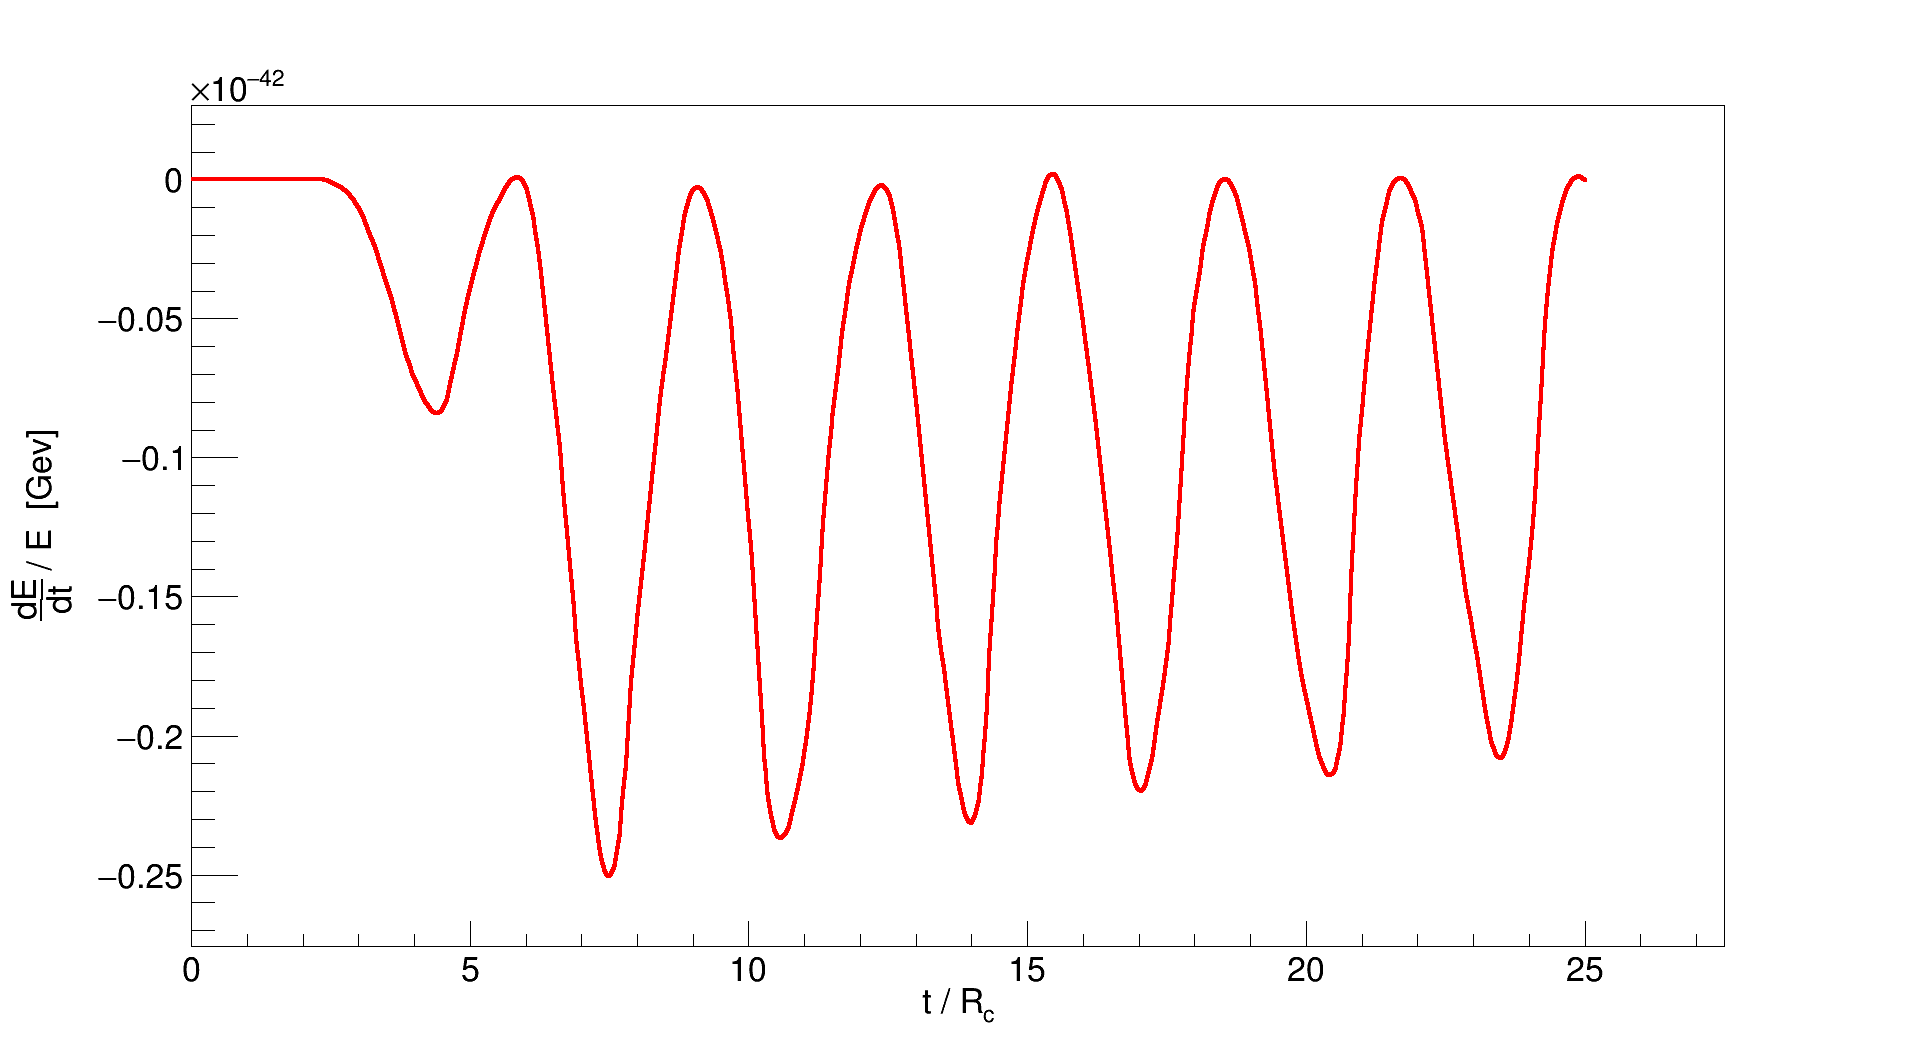
\includegraphics[width=1\columnwidth]{Images/Power.png}
    \caption{The relative power loss $\frac{1}{E}\frac{dE}{dt}$ as a function of $\frac{t}{R_c}$, computed at $r=5R_c$, measured in GeV. Here we have defined negative values as the energy lost by the object.}
    \label{Power}
\end{figure}
In Figure \ref{Power} we see the relative power radiated by the object as a function of relative time $\tau$. Averaging over one period, we get $\left\langle \frac{1}{E}\frac{dE}{dt} \right\rangle \approx 10^{-43} $ GeV, which, when converting back into SI units, is equivalent to $\left\langle \frac{1}{E}\frac{dE}{dt} \right\rangle \approx 10^{-19} s^{-1}$. This value is two orders of magnitude higher than predicted for a similar configuration for the chameleon field \cite{Silvestri:2011ch}.

In order to see how this compares with other dissipation mechanisms, we will compare this result to the emission of gravitational waves from binary systems. To do this, we will want to see how the energy loss of a binary system relates to its period decay.

We can write Kepler's 3rd law as
\begin{equation}
    P = \left(\frac{4\pi^2}{G\left(m_1+m_2\right)}\right)^{1/2}a^{3/2},
    \label{Kepler3law}
\end{equation}
where $P$ is the orbital period, $a$ is the semi-major axis of the orbit and $m_1$ and $m_2$ are the masses of the orbiting bodies. 
We can also write the gravitational energy of a binary system as 
\begin{equation}
     E = -\frac{G\left(m_1m_2\right)}{2a}.
     \label{Gravitenergy}
\end{equation}
~~Taking the time derivative of both Eq.~\eqref{Kepler3law} and Eq.~\eqref{Gravitenergy}, we can compute $\Dot{E}/E$ and $\Dot{P}/P$. Comparing both equations we conclude that
\begin{equation}
    \frac{\Dot{E}}{E} = -\frac{2}{3}\frac{\Dot{P}}{P}.
    \label{periodloss}
\end{equation}
~~This equation allows us to compute the relative energy loss of a binary system from its orbital parameters. Using the data available for the period variation of binary systems, namely the Hulse-Taylor binary and the binaries in Table 7 of Ref.~\cite{Will:2014kxa}, we find that the relative power loss of binary pulsars varies from $\mathcal{O}(10^{-16})s^{-1}$ to $\mathcal{O}(10^{-18})s^{-1}$. Therefore, we find that the energy loss due to scalar waves' emission is subdominant when compared to the one associated to gravitational waves, making the former difficult to detect, as far as this type of systems is concerned.

%%%%%%%%%%%%%%%%%%%%%%%%%%%%%%%%%%%%%%%
\section{\label{sec6}Conclusions}
%%%%%%%%%%%%%%%%%%%%%%%%%%%%%%%%%%%%%%%

We have conducted a study of the symmetron mechanism in the Newtonian limit. 
In this approximation, we were able to obtain its governing equations and study its behaviour near compact massive objects.

In our model, we were able to observe the behaviour of the symmetron and its screening mechanism around a compact astrophysical object with similar dimensions as an average star.
Having solved the equations of motion both through an analytical approximation and a numerical solution, we could clearly see how regions of high matter density suppress the symmetron field, allowing it to remain undetected by local gravity tests.

Having obtained the static profile of the field, we then obtained its time dependent profile near a radially oscillating object. 
As expected, these radial pulsations originate ripples in the field surrounding the object. 
These ripples took the form of waves which decay at a rate of $1/r$, as expected for a spherically emitting source.

These waves in the symmetron field carry away scalar radiation with them, this in turn causes the object to lose energy around the order of $\mathcal{O}(10^{-19}) s^{-1}$ of its total energy, much higher than the value obtained for the chameleon mechanism in Ref.~\cite{Silvestri:2011ch}. However, this value is still lower than known rates for binary pulsars, meaning these scalar waves are as of yet undetectable.

This extra energy loss due to symmetron field oscillations could result in a potentially higher energy loss rate for a binary system than predicted by General Relativity, as the system would emit both gravitational waves and symmetron oscillations. 
This deviation from General Relativity could be an avenue through which we might be able to test the existence of these fields.

Despite the simplicity of our model, it gives us some insights into the behaviour of the symmetron and gives rise to predictions that could possibly be tested, as well as lay the groundwork for a more in depth study of the model.
In this paper we worked in the Newtonian limit, ignored relativistic effects and worked with a very crude model of tidal deformation. 
In the future, it would be useful to work with a model which takes these effects into account in order to obtain a much more reliable result. 

%%%%%%%%%%%%%%%%%%%%%%%%%%%%%%%%%%%%%%%
\section*{\label{sec7}ACKNOWLEDGMENTS}
%%%%%%%%%%%%%%%%%%%%%%%%%%%%%%%%%%%%%%%
SF would like to thank Javier Rubio for the supervision and guidance during the development of this project, as well as the COSTAR team for their feedback on the work.


\bibliographystyle{unsrt} 
\bibliography{bibli} 

\end{document}



